\chapter{绪论}
\section{研究背景}

为了提高导弹的机动性和突防能力,作为导弹动力装置的发动机,要求其具备推力控制,特别是推力随机控制的功能。推力调节技术是固体火箭发动机的一个重要研究领域,与推力预定的发动机(如单室双推力、脉冲发动机等)相比,前者更能合理地分配推进剂能量,根据工作需要调节其推力,这是未来固体火箭发动机的发展趋势。实现推力的随机控制将意味着固体火箭发动机技术的重大突破。从20世纪60年代起,国外为可控推力固体火箭发动机的理论和实验研究作了大量的工作\cite{anon:53},探索出了很多技术途径和设计方案,有的已经进入实际使用阶段,如美国三叉戟导弹末助推系统、前苏联研究的胶状推进剂发动机方案等。1993年以后,美国为满足战区导弹防御系统(TMD)的需要,对小型推进系统进行了大量研究。\cite{bhutta:90jsr}TMD拦截器必须以最少的发射单元和导弹数量覆盖大的作战空域,并防御近距离或远距离来袭的目标群,这就需要一种完全可控的轨控、姿控系统来控制拦截器的机动飞行,通过侧向推力修正预测拦截误差并制导动能弹头直接碰撞目标,以进行有效的拦截。美国航空喷气公司在证明固体姿轨控系统具有与液体姿轨控系统同样灵活性的同时,指出固体姿轨控系统更安全可靠,并可降低成本。

通过改变喷管喉部面积来调节推力是固体火箭发动机推力调节技术的一个研究分支。\cite{bhutta:90vra,bhutta:90cp}在固定喷管型面的条件下,改变喉部面积的方法主要有机械和流体喷射两种方法。目前在固体火箭发动机上采用的机械方法主要是带可移动的喉栓(针栓),通过喉栓的移动来改变喉部面积。该方法的缺陷是驱动喉栓的传动伺服机构尺寸和质量通 常都较大,因而主要适用于小型的固体火箭发动机。

(流体喉部喷管的应用广泛、优点突出)“流体喉部喷管”概念是指通过二次流体喷射,使二次流与主流相互作用从而改变主流的喉部形状和流通面积(流体喷射方法)。流体喉部方案是在喉部附近与主流逆向的喷入二次流体,通过二次流体的挤压和增加流阻使主流流通面积减小(见图1-2(b)),通过调节二次流工质(气体或液体)参数(流量、压强或工作脉宽)从而实现对主流喉道面积大小的控制。最早,美国NASA和空军共同开展了一项名为“射流注入喷管技术(Fluidic Injection Nozzle Technology-FLINT)”的研究计划[17-31],针对该方案在航空发动机上的应用进行了大量研究,并把该技术列为未来先进无人机和战机喷气推进系统的首选。研究表明该种流体喉部喷射方案具有以下特点及优点:(1)该方案没有移动部件,可靠性高;(2)可整合喷管扩张比控制和矢量控制系统,使发动机系统简化。二次流如果在喉部对称的喷入则起到调节喉道面积的作用;如果在喉部附近非对称的喷入则会使喷管音速面倾斜,使主流在亚音速区就产生偏转,从而改变推力的方向;(3)上述流体喉部音速面倾斜诱导矢量控制要比在扩张段喷入二次流的激波诱导矢量控制效率要高,并且推力损失小;(4)二次流的排出本身可提供额外的推力。\cite{blottner:70cp,miner:75ncr,moss:90pc,sutton:85ar,thoman:66phd}

流体喉部喷管技术在航空发动机上的成功应用和验证,对把该技术应用于固体火箭发动机进行推力随控的研制、发展提供了很好的基础,最近人们又开始关注将该种流体喉部喷管技术应用于火箭发动机上。世界第三大军品公司英国BAE System公司2012年与新南威尔士大学合作,对固体火箭发动机的流体喉部特性、关键技术方案进行了初步评估和研究;认为固体流体喉部喷管可以和二次流矢量控制系统结合,可同时实现推力大小和方向调节,从而可以发展出一套更经济、简单实用的固体火箭发动机推力调控系统。英国BAE System公司这一应用思路与著者更早前在2009-2011年间对固体火箭发动机流体喉部系统的研究结论和思路不谋而合。

虽然流体喉部喷管技术仍是一项正在发展中的技术。但可以预见,该技术的发展和突破将会对发展新一代隐身无人机矢量喷管、扩张比可调的航空发动机、流量可控的固体燃气发生器、推力大小和方向随控的固体火箭发动机方面起到重要促进作用;同时也将给上述领域提供一种技术储备,图1-4里列举了流体喉部喷管技术的应用前景。

\section{喷管阻尼效应}
线性稳定性主要研究小扰动振幅的变化规律,主要基础为燃烧室内的一维波动方程。燃烧室内压力$P$可表示为:
\begin{equation}
P=\dot{p}+p_0 e^{\alpha t} e^{j(\omega t+hx)}\label{eq:pressue p}
\end{equation}
若$\alpha>0$,小扰动有增长趋势,则燃烧不稳定;若$\alpha>0$,则小扰动有减弱趋势,燃烧具有稳定性,其增长常数α可表示为各种增益、阻尼效果之和,如式\ref{eq:zengyi}所示。
\begin{equation}
\alpha=\alpha_{pc}+\alpha_{vc}+\alpha_{dc}+\alpha_n+\alpha_p+\alpha_{mf}+\alpha_{g}+\alpha_{w}+\alpha_{st}\label{eq:zengyi}
\end{equation}
式\ref{eq:zengyi}中的各个系数依次为压力耦合响应系数、速度耦合响应系数、分布燃烧增益系数、喷管阻尼系数、惰性微粒阻尼系数、平均流作用系数、气相阻尼系数、壁面耗散阻尼系数与结构阻尼系数。只要各个常数都得到了确定,预估发动机的稳定性就具备了可行性。固发燃烧室内常见的阻尼与增益如图\ref{fig:zengyiyuzuni}所示。
\begin{figure}[htbp]
	\centering
	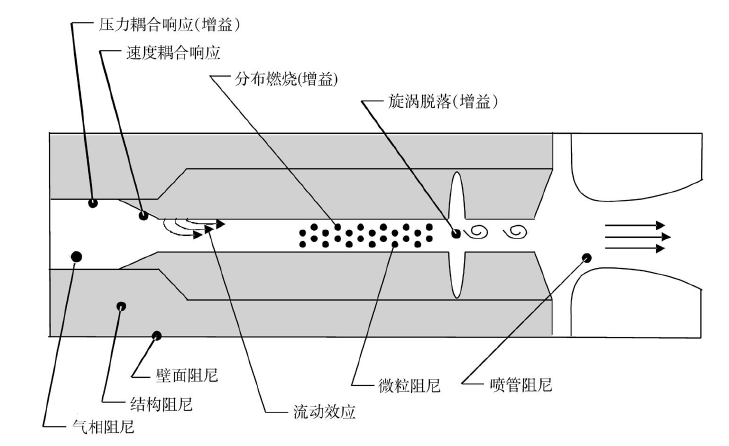
\includegraphics[width=0.7\linewidth]{figures/zengyiyuzuni}
	\caption{固体火箭发动机中常见的增益与阻尼}
	\label{fig:zengyiyuzuni}
\end{figure}
喷管阻尼是固体火箭发动机总阻尼中研究时间最长时间最深的一部分,也是占总阻尼中最大的一部分。我们可用喷管声导纳函数来表征它的大小。在纵向振型以及横向/纵向混合振型中,声能在喷喉处会被吸收或者辐射掉一部分。国内外对该项阻尼的理论研究已经达到了一个相对完善的高度。喷管阻尼决定于燃烧室中产生的扰动以及喷管壁和沿着喷管变化的平均流量两大方面的综合作用。如果喷管流动画成“派”形图的话这个复杂的相互作用过程也许可以更好的被理解,每个派形图都以不同的横截面积以及不同的平均流量性质为特征,并且每个派形图都互相依附(见图1-2)。当一个波从一个派形图移动到另一个派形图的时候,它的一部分被反射了,一部分由于平均流量和管道面积的改变而透射了出去。当波以音速到达喷管喉部时,反射就不再发生,入射波被平均流带出喷管。这些燃烧室中的复杂反应通常由一些适当的边界条件来描述,而这些边界条件也用来描述喷管入口面的不稳定流动状态。喷管的边界条件通常由说明特定的喷管声导纳Y来确定,Y则由喷管入口处的轴向速度扰动和压力扰动的复数比值来确定的。就像后面很快要说明的,喷管声导纳的实数部分的大小极大的影响了喷管入口平面的声能的大小。

喷管阻尼主要由喷管声导纳来描述,对于几何形状简单的喷管,声导纳的计算是可靠的;但对于复杂形状的喷管,特别是潜入式的喷管,主要还是采取实验研究的方法来研究喷管阻尼。 
喷管阻尼损失实质上是一种声场与平均流之间的相互作用。超声速喷管对燃烧室声场不显示开口特性,其原因在于喷管入口段具有很大的压强梯度与温度梯度,即构成了很多声学特性不同的横截面,有效地反射了声波。大部分声波能够被反射,小部分声能可以透过喷管以辐射形式传递到外界。此外,从流出喷管的燃气还能以对流形式带走一部分声能,这两部分声能的耗散将有效地衰减燃烧室内的声能。对于横向振型而言,喷管的阻尼作用非常小,它仅相当于刚性边界条件。因此,喷管阻尼主要是针对轴向振型而言。

喷管耗散的声能可以用喷管声导纳来度量,定义喷管声导纳为分别是喷管入口处的速度振荡和压力振荡。一般情况下,喷管收敛段长度远远小于振荡波长,将此类喷管称为短喷管。短喷管中的流场参数均呈整体型振荡状态,亦即气体在喷管中的流动是准稳态的。虽然气流参数都是时间的函数,但就各个瞬时来讲均能满足准稳态控制方程。

喷管阻尼理论是根据一定简化模型提出的,只能用来预计收敛段光滑过度的喷管。若喷管收敛段几何形状复杂,则理论并不能作出确切的预计,必须通过试验或数值计算来测定其阻尼系数。
\section{国内外研究进展}
\subsection{国内研究进展}
谢侃、王一白、李军伟等人对流体喉部喷管技术的基础问题进行了比较全面的研究,通过仿真和设计喷嘴试验,得到二次流流量比和总压比的关系规律以及有效喉部面积比与流量比的关系曲线。其中有效喉部面积比是用流量系数比来表征的,这是因为喷管通入二次流后有效喉部面积与原喉部面积的比值实际等同于流量系数比(Cd/Cdo),如图\ref{fig:flowvsperciliu}
\begin{figure}[htbp]
	\centering
	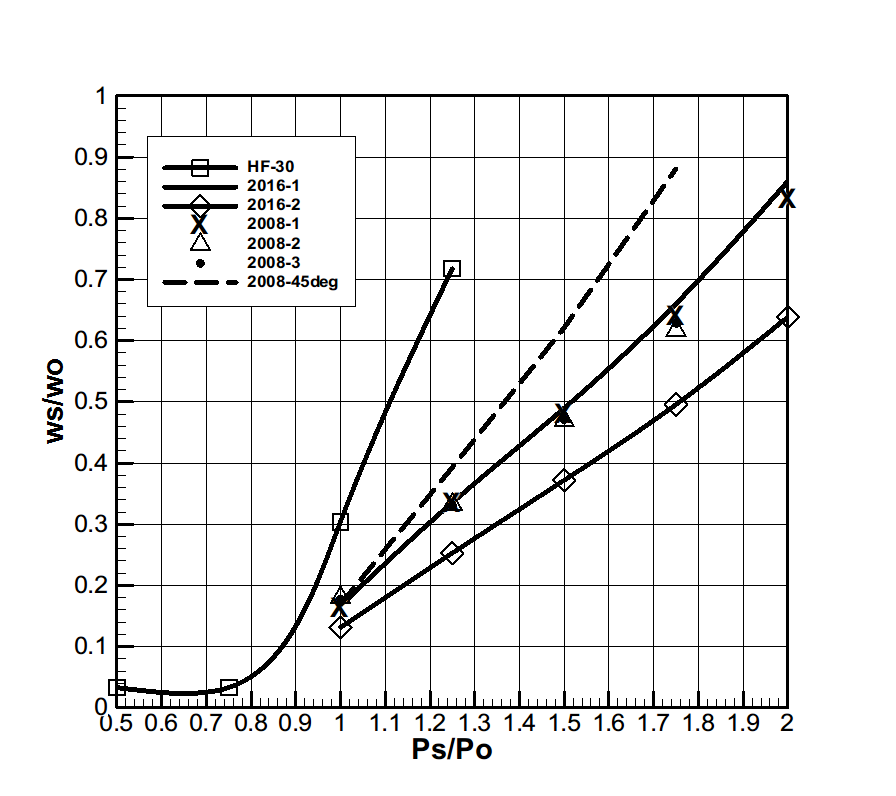
\includegraphics[width=0.7\linewidth]{figures/flowvsperciliu}
	\caption{有效喉部面积比-流量比曲线}
	\label{fig:flowvsperciliu}
\end{figure}

通过多组控制变量实验以及仿真分析,发现二次流总温比、喷嘴个数、二次流流量比、喷射角度、喷嘴面积比及喷射位置是流体喉部有效面积最敏感的参数,其次是喷嘴扩张比、主喷管收缩段的收敛角、布局方案等。而与航空发动机的小扩张比喷管不同,工作时的反压比对固体火箭发动机流体喉部的有效面积影响不大。

连永久总结了射流推力矢量控制技术中亚声速和超声速射流的原理和区别,给出了一些射流推进矢量控制技术的实现方法。对于亚声速喷管采用法向吹气法利用亚声速偏斜产生侧向力,而超声速喷管的吹气法是利用了射流喉部偏斜和激波推力矢量控制。

其中还提到的一种很有前途的反向流推力矢量控制方法,在主喷管外侧有外罩,并使外罩表面和排气喷流之间留下间隙,推力矢量是通过对吸气环的真空控制来实现的,通过激活在上侧外罩和主喷流之间的一台真空泵,在主流上侧剪切层内产生逆向次流,根据coanda附壁效应,主流喷流会产生向上偏转。反流推力矢量喷管的可行性已经被试验结果证明,而且相比机械作动系统具有很多优势,提高了反应敏捷度。

岳明辉、闫东峰等对二次流工质为含有铜粉的高压氮气的热试点火试验进行了分析。结果表明含有铜粉的气态二次流可以催化推进剂的燃烧反应,加快其反应速率,使发动机的推力以及压强响应更加迅速,验证了含催化性颗粒的二次流在固体火箭发动机实现快速响应上的可行性。

苏万兴根据脉冲衰减法原理,总结了仿真和试验结果,分析了不同喉通比下喷管阻尼常数的变化规律(图1-5),解释了在实际固体火箭发动机工作过程中,发动机工作稳定性随工作时间急剧下降,在工作末期出现不稳定燃烧的现象。随着燃面的不断退移,燃烧室通气面积逐渐增大,使得导致喉通比J 随发动机工作进行逐渐减小,继而造成喷管阻尼急剧减小,发动机工作末期,喷管阻尼也达到最小值。


刘佩进、杨尚荣等采用大涡模拟方法研究了工作压强和介质温度对模拟燃烧室中压强振荡的影响,得到的结果表明,相同发动机结构条件下,发动机热试车和冷流实验之间很大程度上存在一致性,因此研究实际发动机流动稳定性可以采用冷流实验的方法,另外还得出了介质温度决定了压强振荡的频率,工作压强决定了振荡的振幅的结论。

孙兵兵、李军伟等基于Buffum冷流试验发动机的二维模型,利用脉冲衰减法,开展喷管阻尼特性数值仿真计算,旨在探索燃烧室工作压强与燃气温度对固体火箭发动机中喷管阻尼特性的影响,发现燃烧室压力变化时,不会带来额外的喷管阻尼,燃烧室内气流速度几乎不变。而燃气温度对喷管阻尼影响很大。

\subsection{国外研究进展}
在1999年意识到脉动喷流结构不仅能增强射流混合,也能增加主流的流阻时,研究人员开始将脉动喷射作为进一步提高扼流性能和减少二次流消耗量的主要手段。该阶段的代表性工作有2000年,P. J. Vermeulen用声振耦合的方法使二次流脉动频率达到了几kHz,采用该方法可方便利用外界的空气,减少由压气机引出的高压空气的需要量[31]。2004年,M. Dziuba和T. Rossman用谐振管的办法将二次流脉动频率提高至了几十kHz[44]。

2007年,D. Baruzzini将流体喉部喷管概念应用在液体火箭发动机上,并提出“有源脉动喷射+无源定常喷射”的组合方案来增强火箭发动机上的流体喉部的扼流性能和减少二次流使用量[42、43]。其中“无源定常喷射”是将液体火箭发动机燃烧室内的高温燃气引出一部份作为入射的二次流使用。这项研究源于美国空军实验室打算评估流体喉部喷管技术对地面发射入轨液体火箭发动机调节喷管膨胀比的优势和可行性。
另外,为找到能产生上述高频脉动二次流的办法,研究人员也开展了大量的理论和试验研究,这方面的代表工作是Patrick J. Yagle[28]和M. Dziuba [44]的研究。他们对利用主动谐振管产生高频音速脉动喷流的方法进行了实验和CFD仿真计算。2005年,M. Dziuba和T. Rossman设计的谐振管用很小流量的高压空气或氦气就能产生15kHz到45kHz的脉动且没有移动部件。

喷管阻尼很早就受到了研究人员的重视,喷管阻尼理论最初是在液体火箭发动机的研制中发展起来的。Crocco为喷管声导纳的研究奠定了基础,发展了喷管声导纳线性理论,在其研究中,假设平均流是一维无旋流,而声波是三维有旋运动,并且在理论分析中考虑了熵波。Zinn基于短喷管理论,对喷管阻尼特性进行了理论预估,并对小尺寸喷管导纳特性进行了冷气试验、试验结果与理论预估结果非常一致,最后提出了喷管阻尼的工程预估公式。

Janardan和他的合作者开展了喷管阻尼试验研究,结果表明锥型收敛段喷管阻尼要优于等曲率型收敛段喷管阻尼。近年来,Anthoine针对含潜入式喷管的发动机开展了理论,试验及数值模拟研究工作,通过燃烧室内的压力振荡特性反映了潜入式喷管对不稳定燃烧的影响,结果表明燃烧室压力振荡与潜入式空腔体积呈线性关系,潜入空腔体积越大,压力振幅越大,也就表明越容易产生不稳定燃烧现象,从侧面反映潜入式空腔对喷管阻尼有较大的影响。

\section{本文主要研究内容}
目前国内外对于普通喷管已经开展了比较多的阻尼实验与仿真研究,而流体喉部技术二次流的施加一定会对喷管的阻尼有所影响,目前尚没有针对于施加了二次射流的喷管的阻尼的专门研究。为了探究流体喉部二次流对喷管阻尼的影响,文章通过实验和仿真的角度,利用稳态波衰减法以及脉冲衰减法的原理,得到了不同工况下流体喉部喷管的阻尼特性;主要讨论了不同的二次流喷射角度以及不同的主流二次流流量比下的阻尼特性变化规律,对比实验仿真结果,相互验证结论可靠性,进一步完善了流体喉部喷管推力矢量控制技术的内容,为这项技术的实际应用提供了参考。


